
%(BEGIN_QUESTION)
% Copyright 2015, Tony R. Kuphaldt, released under the Creative Commons Attribution License (v 1.0)
% This means you may do almost anything with this work of mine, so long as you give me proper credit

This production process manufactures {\it ammonium nitrate}, a principal ingredient of synthetic fertilizer, from the chemical combination of nitric acid and ammonia:

$$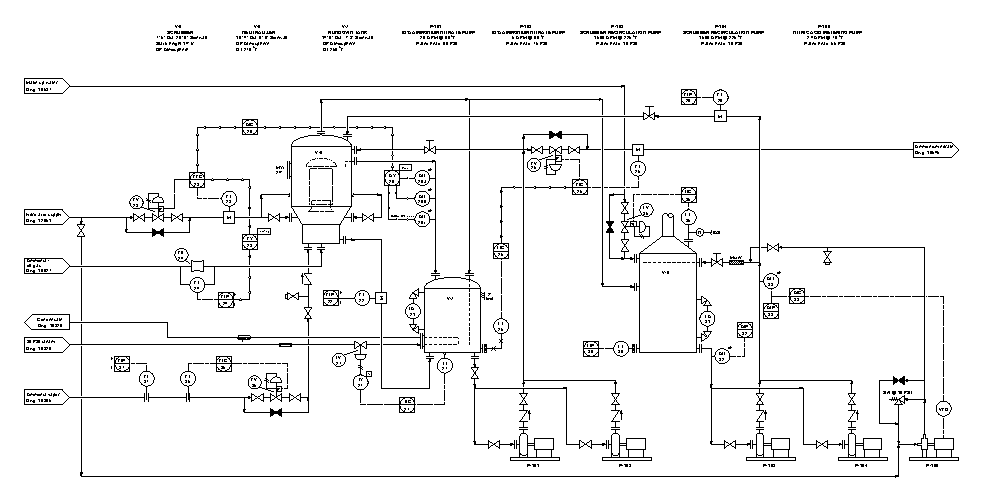
\includegraphics[width=15.5cm]{i0008rx01.eps}$$

Examine the level control system for the scrubber vessel (V-5).  Suppose you were informed that the make-up water header supply pressure tends to vary significantly, and that this was acting as a load in V-5's level control loop.  Explain how you could add cascade control to that level control loop to better manage swings in make-up water supply pressure.

\underbar{file i01277}
%(END_QUESTION)





%(BEGIN_ANSWER)

Cascade control works by adding another controller before the final control element, taking setpoint orders from the original loop controller to ensure the manipulated variable holds to that value.  In this application level controller LIC-35 directly controls valve LV-35 to admit make-up water to the scrubber as needed to maintain a constant level in that scrubber.  Water supply pressure is a load to level control because changes in water supply pressure will directly affect flow rate into V-5 for any given valve position, forcing level controller LIC-35 to compensate as it sees liquid level drift off of setpoint.  

\vskip 10pt

To add cascade control to this application, we would first need to add a flowmeter to the make-up water line so that we could monitor the rate of water flow into V-5.  Then, we would add a flow controller (FIC) to the loop, sensing flow from the new transmitter and taking the output of LIC-35 as a remote setpoint.  The control valve (LV-35) would now be driven by the output of the flow controller rather than by the output of the level controller.
 
\vskip 10pt

Assuming signal-to-open action for LV-35, the new flow controller would need to be configured for {\it reverse action} (i.e. commanding LV-35 to close down if flow exceeds the setpoint given by LIC-35).

%(END_ANSWER)





%(BEGIN_NOTES)


%INDEX% Control, strategies: cascade
%INDEX% Process: ammonium nitrate production (realistic P&ID shown)

%(END_NOTES)


